\documentclass[10pt, a4paper]{report}
\usepackage[utf8]{inputenc}
\usepackage{lscape}   % Make a page in landscape format \begin{landscape}
\usepackage{colortbl} % To color table cells
\usepackage{color} % Able to change textcolor
\usepackage[table]{xcolor}
\usepackage{longtable}
\usepackage{graphicx} % Able to add pictures
\usepackage{parskip}  % Separate paragraphs with a blank line
                      % rather than using indentation
\usepackage{hyperref} % Support for hyperlinks
\usepackage[protrusion=true,expansion=true]{microtype} % Improve justification
\usepackage{subfigure}
\usepackage{hyperref}
\usepackage{caption}
\usepackage{float}
\usepackage{afterpage}
\usepackage{lipsum}
\usepackage{wrapfig}
\usepackage{enumerate}
\usepackage{natbib}

\hypersetup{%
    pdfborder = {0 0 0}
}

\begin{document}

	\begin{titlepage}
\begin{center}

	{\Huge ``Can You Keep a Secret?''\\ [0.4cm]
	- A study of Android Unlock Patterns} \\[1.5cm]

	%Can you keep a secret?
	%Tell me who you are, and I will know your password.

	{\Large TDT4501 - Project Thesis} \\[2.0cm]
	{\Large Marte Dybevik Løge} \\ [0.5cm]
	{\Large Norwegian University of Science and Technology}\\

	\vspace{3.0cm}

			
\includegraphics{pics/ntnu-logo2.png}

	\vspace{3.0cm}

	{\Large Submission date: Desember 2014} \\[0.2cm]
	{\Large Supervisor: Lillian Røstad} \\ [0.2cm]
	{\Large Co-supervisor: Per Thorsheim} \\ [0.2cm]
	{\Large Keywords: graphical passwords, mobile security, Android}


\end{center}
\end{titlepage}\clearpage
	\section*{Abstract}
  
  Since the first proposal for a graphical password around 1996, a variety number of graphical password schemes have been proposed. The proposed graphical password schemes were motivated by the promise of improved password memorability and thus usability, while at the same time trying increase the security.  Psychology studies have recognized that the human brain have a superior memory for recognizing and recalling visual information rather than recognizing and recalling verbal or textual information. Graphical passwords seems as a good replacement of text-based authentication. 

  The motivation for this thesis started by observing the shortcomings with text-based authentication, where people tend to obtain bad habits because of the difficulty of remembering the textual information. People therefore tend to create easily guessed passwords. Password sharing and password reuse are also some of the know habits that people obtain by using text-based passwords. When looking at mobile devices, text-based passwords are not easily typed on a mobile screen. Graphical passwords do not only seem as a good replacement of text-based passwords, but also look like a great authentication method for mobile devices because of the easily interaction with graphical elements on a small touch screen. Graphical passwords on mobile devices are used as a screen lock mechanism to prevent unwanted acess. The history of locking mechanisms was often a solution solely to prevent accidental use, while current mobile phones require protection in order to secure the potentially vast amount of private data that we keep on our mobile devices.

  Android Unlock Patterns is one of the graphical password schemes with an commercial success on mobile devices. The only large-scale study that have conducted quantified the security of peoples choice in patterns. This study aims to take the analysis of people's choice in Android Unlock Patterns a step further by including the human properties that may impact the user's choice in graphical passwords. I believe that graphical passwords are more than just pictures and graphical objects.

  In this thesis there is conducted a literature review of graphical passwords. There is also created a proposal for a research design for further continuation of this work. The research design contains a research strategy, as well as a prototype for data collection. 

  \clearpage
	\tableofcontents \clearpage
	
	%Chapter 1 - Introduction
	\chapter{Introduction}

\section{Background and Motivation}
    
  % In todays society we're addicted to our mobile devices in our every day life. Mobile devices are not just a communication tool for calling and texting, but also an important tool for every day tasks like doing our work, reading mail, pay our bills and keeping up with our social life. Our whole life is contained in one device! When such a small device is so imortant, it makes it vurnerable. How do we secure it?

  % %Information security have become a critical concern from a business point of view

  % There are many different security tips for mobile devices, but the most imortant of them is locking your device with a password. There are many different password schemes, but the most commonly used password schemes are PINs, passphrases and graphical passwords.

  % The interest in graphical passwords started by the assumption that pictures are easier to remember and more secure than words and numbers. Google's Android platform released the  functionality for Unlock Unlock Patterns in 2008. The Android Unlock pattern is a graphical password schemes that asks the user to make a pattern on a 3x3 grid by making a patten of connected nodes. Since its relese there have been a lot of discussion of its security, but few researchers have done a scientific reseach on this. The problem is not just the theoretical password space, but the password space in practice.

  % In 2013 a research group conducted the first large-scale user study on Android Unlock Patterns \cite{Uellenbeck}. The outcome of the research was a analysis of 2900 collected Android Unlock Patterns. They found a lot of bias in the pattern making process cocluding that the schemes are less secure than its theoretical security.

\clearpage
\section{Research Questions and Goals}

The aim of this project is to design an experiment for collecting graphical passwords set by different user types that further will be used in my master thesis the following spring. In the experiment it will be collected passwords, as well as information about the users creating the passwords. Before designing the experiment this thesis will include a detailed state-of-the-art study on passwords. In order to understand the human factors that impacts how people make their passwords, this thesis will also include a study of the psychological aspects that connects humans and passwords. This are covered in my research questions below:

  \subsection*{Research Questions}

    {\bf RQ1: What is the status of current research on graphical passwords? } \\
    Research are always moving forward with new hypothesises and new results in the field. In order to do a research is imortant to know the relevant work as well as avoid answearing questions that already have been aswered.
    
    {\bf RQ2: What human factors may affect our choice of passwords?} \\
    Passwords are human-chosen secrets that are only connected to you as a person. When the secret are created you might create a password that are a association to something you know or recognice; passwords are more than just words and numbers. It is important to study the bias introduced in the password making process that can be a cause of human factors. Psychology are a field of study that might can give a understanding of how we think and give an explanation of why we make the choices that we do. 
    
    {\bf RQ3: How should an experiment to collect graphical passwords set by varoius user types be designed?} \\
    It is important to consider the biases that can be introduced as a cause of the experiment design. The design have to consider what data that needs to be collected and how the data should be collected. It is also important to consider the diversity of the data in order to be able to get good resluts from the analysis. The result will be a detailed design on the experiment that will be conducted in the following spring. 

\section{Research Method}  

\section{Thesis structure}





% \item To what extent can graphical elements like colors, shapes, and objects infuence the end-users choice of passwords?
% \item How is features describing the end-user picked, and how do the features relate to end-user's choice of passwords?
% \item Kan grafiske elementer påvirke brukerens valg av passord?
% \item Hvilke kjennetegn ved en person kan gi utslag på valg av passord?
% \item Hvordan skal innsamling av passord skjer for å ivareta datasamlingens pålitelighet?

% \item To what extent can we relate existing research on users choice of alphanumeric passwords to users choice of Android unlock patterns? 
% \item How should passwords from end-users be collected in order to preserve the reliability of the data? 
% \item In order to analyse collected Android unlock patterns, how much data is needed to be collected, and how should the diversity of the data look like?
% \item What kind of data should be included in the data model?
% \item How should the data model be designed in order to cover relevant data for the analysis of the collected data?  
% \item What are the status on research on mobile security?
% \item How should passwords from end-users be collected in order to preserve the reliability of the data? 


	% Chapter 2 - BackgroundTheory
	  \chapter{An Introduction to Authentication Mechanisms}
  \label{chap:background}
  
    This chapter is an introduction to authentication mechanisms. Section~\ref{sec:authentication} is an introduction to the categorization of existing authentication mechanisms. The different authentication mechanisms will provide a description, as well as it attached benefits and drawbacks of using a particular authentication mechanism. Section~\ref{sec:entropy} provides an introduction to fundamental aspects of security and authentication. Section~\ref{sec:shortcomings} is an evaluation of the text-based authentication and its shortcomings.

  \clearpage

  \section{Authentication} \label{sec:authentication}

  Authentication is the process of verifying whether a particular individual or a device should be granted access to a system or application running on a device \cite{IPAS}, e.g. verifying that you are the person that you claim to be.

  There are various authentication schemes described in the literature, but they can all be grouped by the following characteristics:

    \begin{itemize}
      \item Who you are
      \item Something you have, and
      \item Something you know
    \end{itemize}

    \subsection{Biometric Authentication}
    Biometric authentication has the characteristics of ``who you are''. Biometric authentication refers to verify a person's identity based on physical or behavioral characteristics of an individual \cite{biometrics, biometrics2}. Biometric authentication is different from other authentications schemes because:

      \begin{itemize}
        \item the biometric password cannot be lost nor forgotten,
        \item biometric passwords tends to be difficult to copy, share and distribute, and 
        \item the person being authenticated needs to be present in the authentication process
      \end{itemize} 

    Physiological biometrics uses the physiological characteristics of an individual in the authentication process. The verification uses unique characteristics of a human, e.g. physical parts of the body that are unique as fingerprints, face, iris, hand and finger geometry, and DNA. Behavioral biometrics analyzes how a person performs different activities, e.g. applies pattern recognition techniques for activities like keyboard writing, talking and handwriting.

    The benefits achieved by using biometric authentication is that each password is unique and only connected to one person. When using an authentication scheme that requires the user to use something they know in the authentication process, it might be forgotten or shared. Biometric authentication cannot be shared, nor copied. The user does also not need to remember the biometric password because it is a part of you.

    There is also some drawbacks with biometric authentication. The implementation of biometric authentication is more complicated to implement because of the hardware needed. Other aspects of biometric authentication are the reliability. Many of the existing equipment used at, for instance, an airport only use images of the finger, and many do not detect if a real fingerprint is used. The same is used for face recognition where it is only used algorithms for authenticate the image of the face. In the case of fraud, you can categorize it as identity fraud because a part of you used for authentication is stolen. It is, therefore, a high responsibility for owners of a system using biometric authentication to store the data in a safe way.

    \subsection{Token-based Authentication}
    In a token-based authentication process the user uses ``something you have'' that is often stored on a physical device. Token-based authentication is often combined with a ``something you know'', making a strong authentication by combining two or more authentication characteristics. In many banking systems you have to use more than just something you know, but also ``something you have'', like a one-time password to pass the authentication process. The one-time password is a password that is generated on the physical device. This is an extra layer of security, because even if someone steals or know your password, he or she still can't get access to your banking account because he or she also would need your security token.

    One drawback of using token-based authentication is that the user must carry the token with them. Without the token, the users are not able to be authenticated. 

    \subsection{Knowledge-based Authentication}
    `Something you know'' is often used in the classical login situation where the user has to remember a username/password to get access to the system or device. Some of the commonly used passwords schemes are PIN's, alphanumeric passwords and graphical passwords that all are passwords with the characteristic of ``something you know''.

    One of the benefits by using knowledge-based authentication is that this is the authentication type that is mostly used for authentication. Since most systems use it, people are also familiar with how it works. The technical solutions do also not require any hardware and can be implemented at a low cost.

    One drawback is that the users needs to remember the password used in the authentication. Since the knowledge-based authentication is used in many systems, especially on Internet, the users are also required to remember all the various passwords on different systems. Requiring the users to remember the password often causes the users to select simple password that is easy to remember, and therefore might be easy to guess.

    There are three different knowledge-based authentication types:

    {\bf PIN's} Personal identification number is a numeric password. The PIN was first introduced in the first ATM in London in 1967 as an efficient way for the banks to authenticate their customers \cite{Bonneau1}. PINS are often a four-digit number. The benefit with a PIN is that it is a short sequence. The drawback is that people often tend to choose a sequence of number that are easily memorized. A known selection of PIN is to select a date that is easily remembered like the date of birth. Such choices are well known to attackers, and such PIN codes can easily be guessed.

    {\bf Alphanumeric passwords}
    The word ``Alphanumeric'' is a composition of the phrase ``alpha'' (as in alphabet), and ``numeric''(as in numbers). The alphanumeric password may also contain special characters, so in short an alphanumeric password is a mix of all writable characters. This is rapid used in systems using a combination of username and password. One drawback is that, like with PINs, people often choose a sequence of characters that is connected to the person. A know strategy for passwords selection is to choose words that are associated with the system, or words that are closely related to the person.

    Systems using alphanumeric passwords often requires the users to change the password at specified intervals. This often causes users to choose a simple password and only make a small change to the password when a change is required. If an attacker knows the password policy, it is possible to make a dictionary with likely used words and characters.

    {\bf Graphical passwords}
    A graphical password has the characteristics of ``something you know'', but instead of using letters and numbers it uses graphical elements. Graphical passwords were proposed as an alternative to PINs and alphanumeric values because humans tends to remember graphical elements better than letters and numbers. A variety of graphical passwords schemes has been created over the past years. Biddle et al. have collected research of the past decade on graphical password schemes \cite{Biddle}, dividing the schemes into three categories:

      \begin{itemize}
        \item Recall-based authentication
        \item Recognition-based authentication, and 
        \item Cued-recall authentication.
      \end{itemize}
      
    Recall-based graphical passwords are often referred to as drawmetric systems \cite{DeAngeli} because the user are are reproducing a secret drawing. The password is usually drawn in a grid or a blank canvas, requiring the user to reproduce the secret password from its memory.

    Recognition-based passwords are often referred to as cognometric systems \cite{DeAngeli} because the user recall a secret drawing or sequence of drawings.

    Cued-recall is often referred to locimetric systems \cite{DeAngeli}. With cued-recall authentication typically require the users to remember and target a particular location within and image. This is a version of a recall-based authentication but helps the user with the recall by showing an image and not just a grid or canvas. It is also different from the recognition-based approach because the user needs to identify specific locations in the picture as a whole. 
    
  \section{Key Security Aspects in Authentication} \label{sec:entropy}
  In order to be able to evaluate the security of different password schemes, this section will give a brief introduction to key security aspects of knowledge-based authentication, and hereafter called passwords. In terms of security, the primary goal of authentication is to provide protection for its intended environment in order to avoid security attacks. A password, regardless of format, is a secret a user needs to use in order to to grant access to the system or device. A password should have certain features in order to be secure:

    \begin{itemize}
      \item The password should be hard to guess, meaning that the password should have a high entropy,
      \item The password should be easy to remember for users, and 
      \item The password should remain a secret for the intended user.
    \end{itemize}

  When we talk about security, we often talk about if a password scheme is ``crackable'', meaning that the a password are guessable. When a password scheme is measured to be ``hard to guess'', it is normal to measure the strength of the password scheme in terms of its entropy. The password strength is measured in terms of information entropy, measured in bits. Instead of measuring the security of a password in number of guesses needed to guess the password, we use the base-2 logarithm of the number of guesses, which is the number of ``entropy bits'' in a password. We use the notation L for the length of the symbols in the password, and they are chosen from a set of N possible symbols. The formula for password entropy are:

    \begin{equation}
      Password Entropy = log_{2}(N^{L})
    \end{equation}

  When we say that a password scheme is easy to use it is normal to measure the success rate when writing and remembering a password, e.g. how long it takes for users to write and remember their passwords. When a password is easy to remember, it often refers to a password scheme ability to maintain its usability. As stated, a password that have a higher entropy are harder to guess, but are often obtained by making long passwords. It is well known that humans have a hard time remembering long and complex passwords. Therefore, it is important that a password scheme are supporting the users to make passwords that they can remember, and also are secure.

  When users make their password it should only remain a secret that the intended user know about. A password scheme that lack support of usability often make people do like create simple passwords that are easy to remember, but also easy to guess, or even write down and use the same passwords on multiple systems.

  All of the key security aspects are important to understand when you are studying password mechanisms. The fundamental aspects will be used throughout this thesis in order to be able to evaluate and read research focusing passwords. 

  \section{Shortcomings With Text-Based Authentication} \label{sec:shortcomings}

  User authentication is a central component of security systems. In order to get access to systems, you need to pass the authentication process. Despite the extensive number of options for authentication, text-based passwords remain the most common authentication scheme. The reason they are widely adopted is because they are easy and inexpensive to implement, and users are familiar with the scheme. It is also avoiding the privacy issues raised by biometric authentication and prevent the need for bringing a physical security device that are used in token-based authentication schemes. However, text-based authentication suffers from both security and usability disadvantages. Today, users needs to remember an increasingly number of password, making users adopt bad password habits.

  The term ``habit'' is often a bad thing when talking about security. A habit is often hard to change and are often a predictable pattern. Password reuse is one of the known password habits among users because the human limitation to remembering text-based password. Some users also make simple or meaningful password that are easier to remember, making their passwords vulnerable to attacks. It is a well-known problem that users tend to have an increasingly number of accounts that requires the users to remember yet another number of password on multiple systems and devices. The problem is not just to remember all the password needed, but also remembering which passwords that belong to which account or device. Because of the human capacity for remembering password are causing users to choose weak passwords, as well as reuse the passwords across multiple web pages. In order to understand the shortcomings with text-based passwords, this section will include relevant research on users choices on text-based passwords.

  Password schemes have what is called an empirical password space, and that is the number of possible passwords that a user can make. The problem with many password schemes is that it seems that users don't tend to use the full password space, but only a subset of the possible passwords, e.g. the memorable password space, making the memorable password space less than the empirical password space (Figure~\ref{fig:memorable}). This shows that the security of a password scheme is linked closely to is memorable password space rather than its full password space.

  \begin{figure}[H]
      \centering
      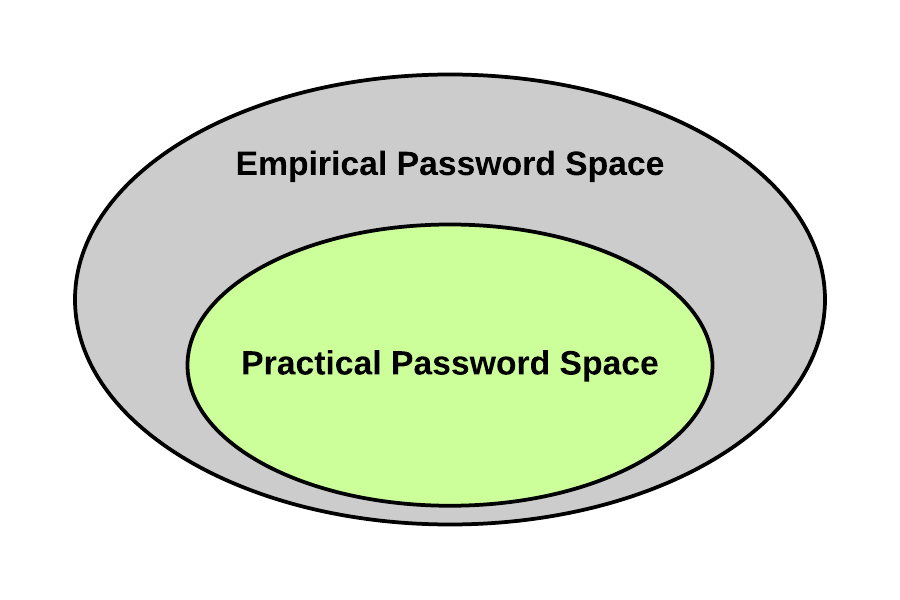
\includegraphics[scale=0.25]{pics/EmpiricalVsPractical.png}
      \caption{Empirical vs. Memorable Password Space}
      \label{fig:memorable}
    \end{figure}

  In a case study of 14.000 Unix passwords, a research group found a 25\% of the passwords were in a group of words forming a dictionary of $3\times10^{6}$ words \cite{UnixPasswords}. This dictionary shows that an attacker can have a relatively high success rate for an attack, despite the fact that there a roughly $2\times10^{14}$ 8-character passwords consisting of digits, and upper case and lower case letters. Due to the limitations of human memory, users often choose passwords that are easier to remember, causing a significant number of user-chosen password to fall into a small dictionary, e.g. practical password space \cite{Tao}. A well-designed dictionary is a tiny subset of the full password space, e.g. theoretical password space, which further can be prioritized according to the likelihood for a password to be chosen. It is, therefore, a commonly stated that the security of a password scheme is related closely to the size of its memorable/practical password space, rather than its theoretical password space. The high success rate of dictionary attack against textual passwords is believed to be strongly related to the recall capabilities of humans and how they choose their passwords, e.g. making meaningful and thus more easily remembered words are selected as passwords.

  One of the first large-scale studies on web password habits was conducted in 2007 by Microsoft research \cite{habits1}. They analyzed web password habits among 544960 Internet users over a period of 3 months. The data was collected from a Windows Live Toolbar, and they observed activities like login frequency. They also gathered information about the users age, the strength of the users passwords, as well as number of unique passwords and its use across different URLs. They observed that a typical user have an average of 7 distinct passwords and that an average of 5 of these passwords was re-used on different web pages. An estimate of the average number of account per user was estimated to be 25 accounts per user, but this would probably be higher since it seven years ago.

  Because of the shortcomings with a text-based authentication, graphical authentication are getting increased attention because it is an alternative to a text-based authentication trying to cope with the memorability and security issues of text-based password. Graphical passwords are using images and visual objects in the authentication instead of text and numeric values. When comparing text against visual objects, the human brain is more capable of remembering images than text. When the human brain is more suited for remembering images, the users might be able to remember more complicated passwords that are not easily guessed. To context where an authentication scheme is used have to be evaluated. Graphical passwords might not fit in all systems, but looks like a good alternative to mobile devices where the user interact with a touch sensitive screen. Typing a long text-based password on a small keyboard on a mobile device is not easy. When using, graphical passwords are easier to interact with on a small mobile screen.


	% Chapter 3 - Litterature Study
	
\section{Structured Litterature Study}

  \subsection*{Planning}

    This section will give a detailed plan for the structured litterature review, as well as building a 
    evaluation protocol for the review. 
    Research should be conducted in order to answer questions that have not been answerd yet. 
    By conducting a structured literature review, I can support my motivation for doing the research, 
    as well as get to know relevant research. 

    \subsection*{Field of Study}

      Before conducting the litterature study, I will do a specification of my field of study in order to
      avoid a unsustainable broad scope. Too broas scope in a litterature study can give to irrelevant searches 
      and it will be hard to find the relevant information needed to answer the research questions. 

      In the figure below I have done a analysis of my field of study. The research will focus on authentication on mobile devices. 
      The type of authentication is screen locks. Finally the inner circle, the most specific topic, is the Android Unlock Pattern. 

      \begin{figure}[H]
        \centering
        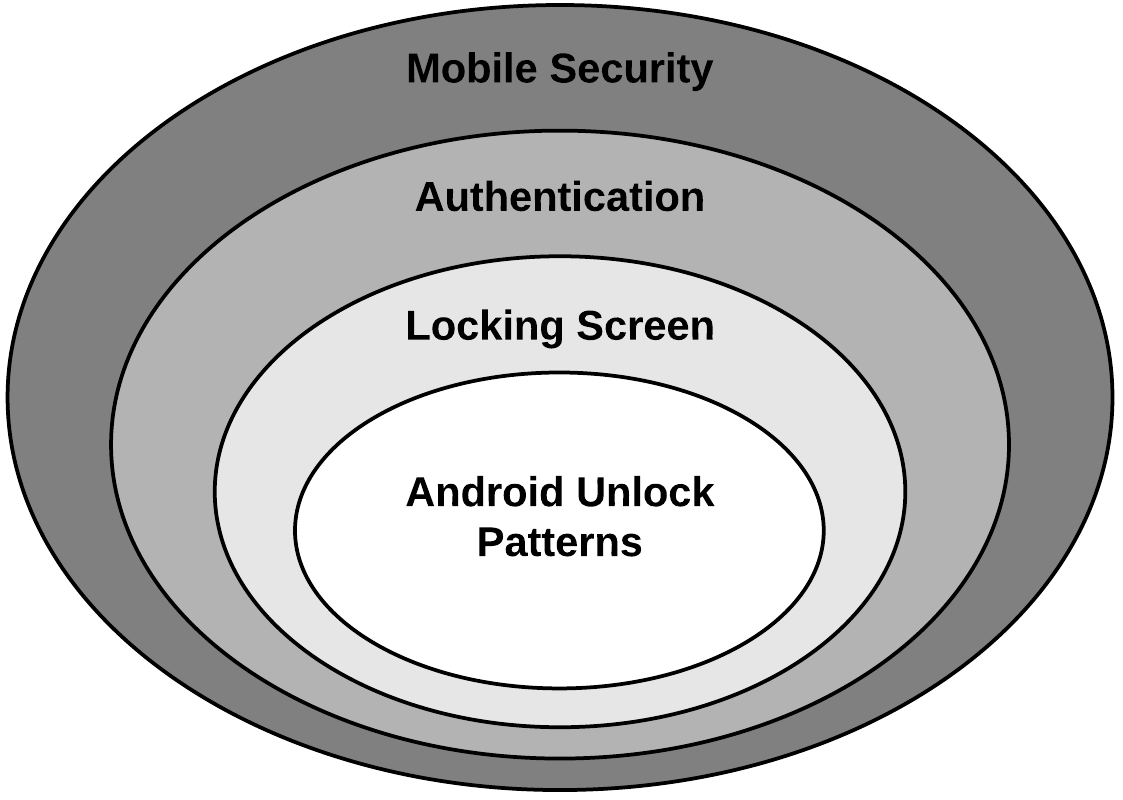
\includegraphics[scale=0.25]{pics/Fieldofstudy.png}
        \caption{Field of study}
      \end{figure}

    \subsection*{Keywords}  

      In the `field of study' I specified a specific scope in order to avoid to broad search space. 
      Inside each of the circles we can get more into details and create specific keywords that I will use in 
      the litterature search. 

      
        \begin{tabular}{ || l | l ||}
          \hline
          {\bf Mobile Security} & \\
          {\bf Locking Screen} &  \\
          {\bf Authentication} &  \\
          {\bf Android Unlock Patterns} & \\ 
          {\bf Psycology} & \\
          {\bf Graphical passwords} & \\
          \hline

          
        \end{tabular}




    \subsection*{Review Protocol}



	
\section{Results from the Litterature Study}

  \subsection{Password habits among web users}

    %Password reuse, frequency of webpage use (login habits), password strength, password policy

  The term ``habit'' is often a bad thing when talking about security. A habit is often hard to change and are often a predictable pattern. Password reuse is one of the known password habits among users. It is a well known problem that users tends to have an increasingly number of account that requires the users to remember yet another number of password across muliple systems and devices. The problem is not just to remember all the password needed, but also remembering which passwords that belongs to which account or device. Because of the human capacity of remembering password are causing users to choose weak passwords, as well as reuse the passwors across muliple web pages. In order to understand the users passwords habits, this section will include relevant research on users passwords habits.

  One of the first large-scale studies on web password habits was conducted in 2007 by Microsoft research \cite{habits1}. They analysed web password habits among 544960 web users over a period of 3 months. The data was collected from a Windows Live Toolbar and they observed activities like login frequency. They also collected information about the users age, the strength of the users passwords, as well as number of unique passwords and its use across different URLs. They observed that a normal user have an average of 7 distinct password and that an average of 5 of these password was re-used on different webpages. The estimate on average number of account pr user was estimated to be 25 account pr user, but this would probably be higher since it 7 years ago. 

  Password habits may be different across different subpopulation in cause of different background or culture. In 2012 Joseph Bonneau released a analysis of 70 million passwords from Yahoo! \cite{Bonneau2}. The data is analysed in terms of guessing rate by using a dictiornary attack. The collected data contained 328 subpopulations. The results showed that there was no ``good'' populations among the collected data, but there was a variation in the population. Demographically, the gender had a small effect in the guessing rate, but it showed that age tended to give effekt where password strength increases across different age groups. The analysis also showed that laguage had a significally effect on the password strength where Indonesian-speaking users were among the weakest subpopulations, and in contrast the German and Korean-speaking users provided relativley stonger passwords. 

  Passwords are not just used in our private life, but also a requirement in a critical concern from a business point of view where the use of authentication for corporate systems, mobile, and room codes plays a major role in normal day of work. In corporate systems users are often promt with the a notification frorcing them to change the password in a specified time interval. The problem with this is that user already have problems remembering their passwords as is. A reseach group conducted a questionnaire survey in a large organization \cite{habits2}. The goal was to get a understanding of password habits in a business point of view. The results showed that the users were promped with password change 7 times a year causing 68\% of the employees to re-use the same password with a minor change in order to still be able to remembering their passwords.

  \subsection{Security habits among smartphone users}

  %Intro
  Users are not only dependent on remembering passwords across multiple web pages and systems, but do also need to remember passwords for our small mobile devices. In todays society we're addicted to our mobile devices in our every day life. Mobile devices are not just a communication tool for calling and texting, but also an important tool for every day tasks like doing our work, reading mail, pay our bills and keeping up with our social life. This trend makes our mobile devices vurnerable in terms of security. To avoid unwanted access, smartphones offers different locking mechanisms. The history of locking mechanisms was often a solution solely to prevent accidental use, while current mobile phones require protection in order to secure the potentially vast amount of private data that we keep on our smartphones. Our mobile devices are in rapidly use, leading users to create and reuse shorter passwords and PINs, or no authentication at all. 

  % The time used on unlocking the phone
  In terms of security it is intersting to look at the use of mobile devices and look at the locking habits among users on mobile devices. It is known that services that are rapidly used have weaker password because of the overhad the user needs to spend on typeing their password. In 2014 a group of reasearchers published a fieild study of smartphone (un)locking behavior \cite{habits3}. Some of the problems with smartphone users tends to be their rapidly use of their phone. When the device are rabidly use, it results in a lot of time unlocking their phone between every use. In the study they found that there was a significant overhead in the time used of unlocking their phone, where the users participated in the field study used 2.9\% (9\% in the worst case) of their time unlocking their smartphone. 
  
  % The use of locking mechanisms
  Smartphones in use today do not require their users to have a locking mechanism on their smartphone. It is well known that users tends to choose to easiet way out and may result in the choice of not having any locking mechanism at all. Based on the result of the overhead in time used on unlocking their phone, a result may be to take the easiest way out by ignoring the vurlerability of not using a locking mechnismn at all. It have been discovered that over 40\% of the users only used a basic ``slide-to-unlock'' mechanism on their smartphone, as well as over 16\% didnt use any locking mechanismns at all \cite{habits3}. This highlights a major bad habit among mobile users. What happens if your mobile is stolen? 

  % Risk vs securtiy
  It is important to understand why people use or not use locking mechanisms on their smartphone. Reseach have covered that the 46.8\% of the paricipants agreed or fully agreed that unlocking their phone can be annoying, but at the same time 95.5\% of the somewhat or fully agreed that they liked the idea that their phone was protected \cite{habits3}. This highlights that the users wants to be secure, but there might be a tradeoff between the time used to unlock the smartphone vs the security risk.








    

    %How many looses their phones?
    %How much do users use their phone (measured in hours)?






  \subsection{Graphical passwords}




  \subsection{Android Unlock Pattern}

    The Android Unlock Patterns are a simplified version of the Pass-Go scheme that was proposed by Tao and Adams in 2008, and can be seen as a successor of the Draw-a-Secret (DAS) scheme. Both Pass-Go, Draw-a-Secret, and Android Unlock Patterns is categorized as recall-based authentication schemes.

    The Android password patterns are a simplified version of the Pass-Go scheme using a 3x3 grid, instead of a 9x9 as the Pass-Go scheme originally was designed. The Pass-Go scheme was inspiered from the chineese board game ``Go''.

    The settings on Android phones provides a default setting for using the Unlock pattern. 
    The rules are simple: 
        \begin{enumerate}
            \item At least four points must be chosen,
            \item You cannot vist the same node twice.
            \item Only straight lines are allowed, and
            \item One cannot jump over point not visited before
        \end{enumerate}

    \begin{figure}[H]
        \centering
        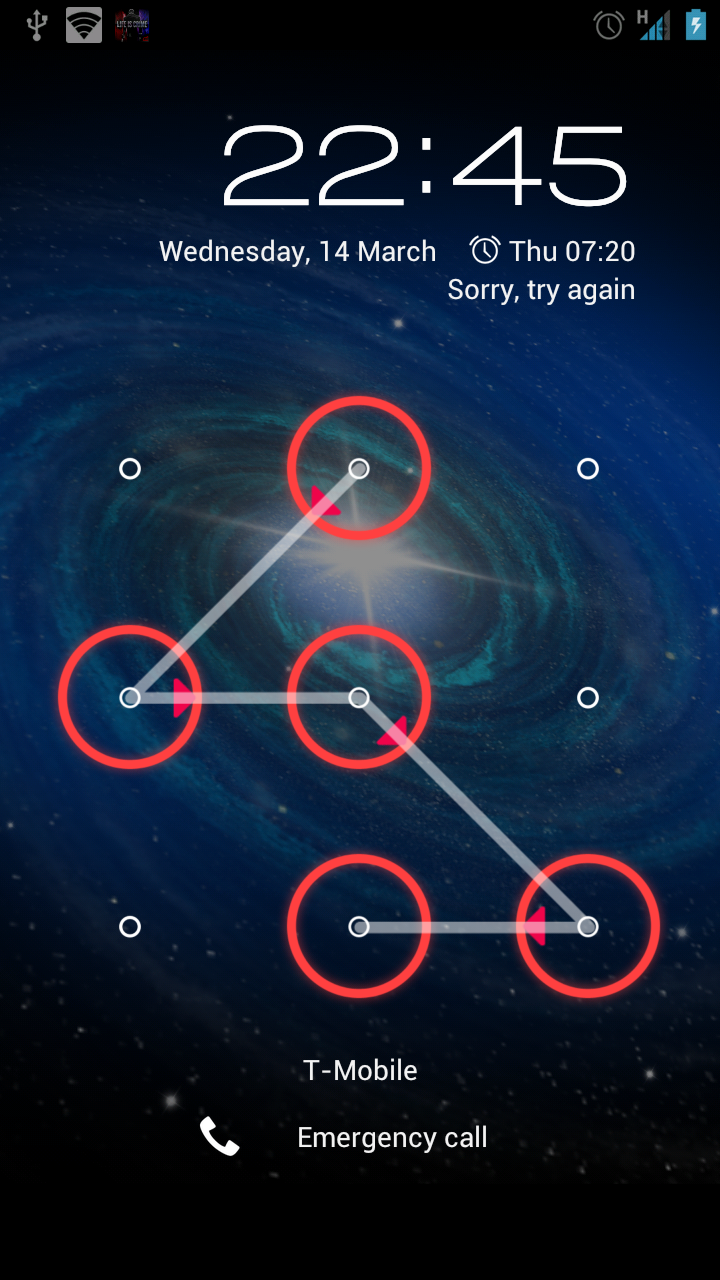
\includegraphics[scale=0.8]{pics/patternLock.png}
    \end{figure}

	%Bibtex
	\bibliographystyle{plain}
	\bibliography{myBib}

\end{document}